\pagebreak
\section{Instructions to run the code.} \label{T4}

\paragraph{}The script needs to be run and should run correctly on any linux environment. However, it has only been tested on a Debian environment. The pre-requisite to run the script is to have git, pip3, python3, aws and docker installed. To make sure the script is executable, the command \verb|sudo chmod +x script.sh| must be executed. Our bash script can then be run as root with the command \verb|sudo .\script.sh|. Out git repository will then be automatically cloned and the \verb|run.sh| script will be executed, which will automatically install all the necessary Python libraries.

\paragraph{}Alternatively, the script can be run manually. To do so, the repository must be cloned using this command:\\\verb|git clone https://github.com/JordMim/LOG8415E.git|. The script will then be located in the directory \verb|LOG8415E/tp1|. The script must be set as executable using the command \verb|sudo chmod +x run.sh|, and can then be run using the command \verb|sudo ./run.sh|.

\paragraph{}When running the script, you'll be asked to setup AWS credentials. If this is your first time using the script, you'll have to do this setup. After that, this step can be omitted, as it will fetch the default credentials saved in AWS.\\

\begin{center}
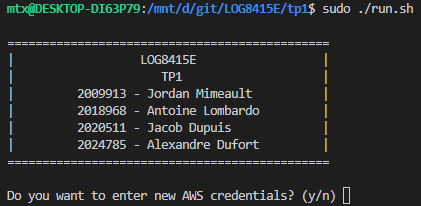
\includegraphics[width=10cm]{Resources/aws_credentials.png}\\
\emph{Figure 4.1 - Execution of command \verb|sudo ./run.sh|}
\end{center}\\

\paragraph{}When AWS configuration is done, you'll be asked what actions needs to be done. There are five options:
\begin{itemize}
  \item Configure AWS Load Balancer, which basically creates all the necessary AWS resources.
  \item Run requests sender, which runs the benchmark.
  \item Fetch metrics, which fetch CloudWatch metrics and export them into JSON and latex format.
  \item Only run benchmark and fetch metrics.
  \item Do everything.
\end{itemize}

\begin{center}
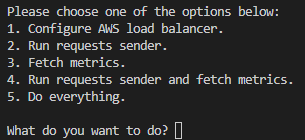
\includegraphics[width=8cm]{Resources/options.png}\\
\emph{Figure 4.2 - Possible options of action}
\end{center}\\

\lef\paragraph{}For each step of the script, the normal output should look like these:

\begin{center}\centering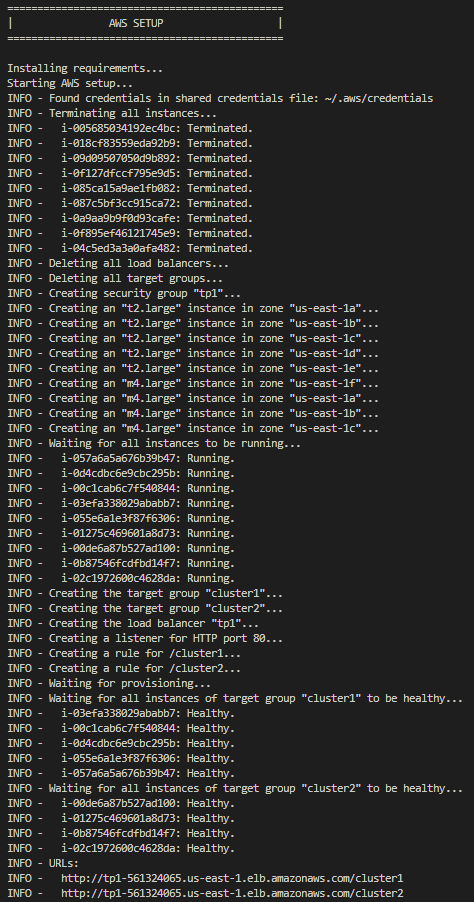
\includegraphics[width=10cm]{Resources/aws_setup.png}\\\emph{Figure 4.3 - Output of the AWS Setup step}\end{center}\\
\begin{center}\centering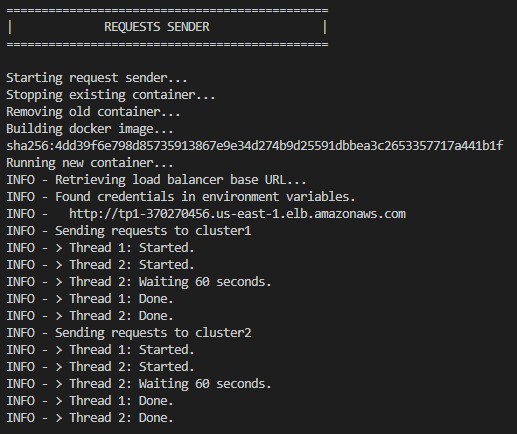
\includegraphics[width=10cm]{Resources/requests.png}\\\emph{Figure 4.4 - Output of the Requests Sender step}\end{center}\\
\begin{center}\centering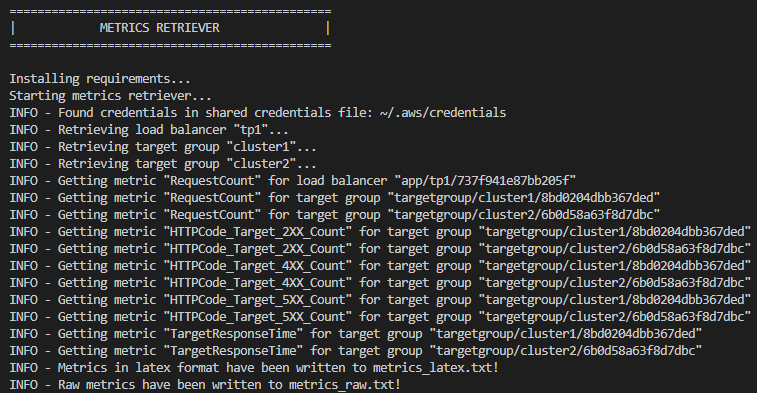
\includegraphics[width=10cm]{Resources/metrics.png}\\\emph{Figure 4.5 - Output of the Metrics Retriever step}\end{center}\\


